% !TEX root = ../main.tex

\chapter{Method}
\label{ch:method}

\section{OpenAI Gym Environments}
\label{sec:environments}
OpenAI Gym offers five environments ready to use in their \textit{classic control} suite: \verb|CartPole|, \texttt{Acrobot}, \verb|MountainCar|, \verb|MountainCarContiuous|, and \verb|Pendulum|. The initial state of each environment is stochastic. Out of all environments OpenAI Gym provides, the classic control environments are considered the easier ones to solve while still being used as baselines in multiple applications. Each environment defines an observation space and an action space. An agent performs some action from the action space and receives an observation describing how the environment's state changed. The information about the environments for this section was taken from the online documentation\footnote{https://www.gymlibrary.ml/}.

\subsection{CartPole}
The \verb|CartPole| environment corresponds to the pole-balancing problem formulated in \emph{Neuronlike Adaptive Elements That Can Solve Difficult Learning Control Problems} (\cite{6313077}). A pole is attached to a cart that the agent can move along a one-dimensional rail. Fig.~\ref{fig:cartpole} shows two possible states of this problem. In the image on the left, the pole is perfectly balanced and upright. The right image shows the pole tilted to the left. Thus, the cart should in principle move to the left to correct the angle of the pole.
\begin{figure}[!ht]
  \centering
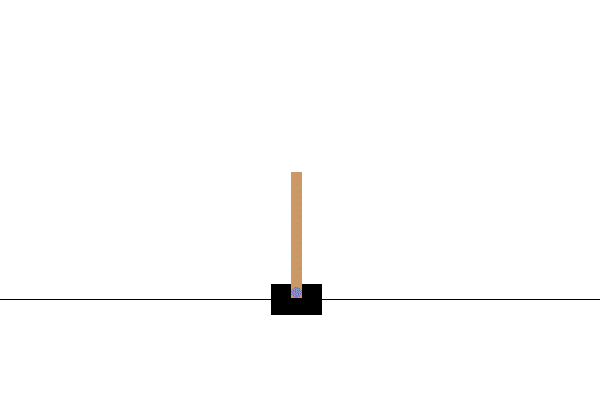
\includegraphics[width=0.4\textwidth]{cartpole} \hspace*{10mm} 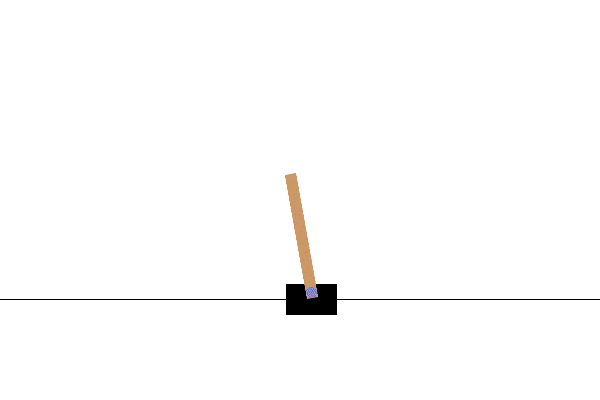
\includegraphics[width=0.4\textwidth]{cartpole_tilted}
\caption[Illustration of the environment CartPole]{
  \textbf{Illustration of the environment CartPole.}
  The image shows two possible states of the \texttt{CartPole} environment. The left image shows a perfectly balanced pole. In the right image, the pole tilts to the left.
}
\label{fig:cartpole}
\end{figure}

\paragraph*{Action Space:} The \verb|CartPole| environment accepts one action per time step and has a discrete action space of \{0, 1\}. The action indicates the direction in which we push the cart by a fixed force, left and right respectively. The actions are described in Table~\ref{table:cartpole_act}.
\begin{table}[!ht]
  \centering
  \begin{tabular}{ |c|c| }
    \hline
    Action & Description \\
    \hline
    0 & Push cart to the left \\
    1 & Push cart to the right \\
    \hline
  \end{tabular}
  \caption[Action space of the environment CartPole]{
    \textbf{Action space of the environment CartPole.}
    Description of all possible actions for the \texttt{CartPole} environment.
  }
  \label{table:cartpole_act}
\end{table}

\paragraph*{Observation Space:} For \verb|CartPole|, we receive four observations informing us about the position and velocity of the cart and the pole. Table~\ref{table:cartpole_obs} shows all observations with the range of the corresponding values.
\begin{table}[!ht]
  \centering
  \begin{tabular}{ |c|c|c| }
    \hline
    Observation & Min & Max \\
    \hline
    Cart Position & -4.8 & 4.8 \\
    Cart Velocity & -Inf & Inf \\
    Pole Angle & $\smallsim$ -0.418 rad (-24°) & $\smallsim$ 0.418 rad (24°) \\
    Pole Angular Velocity & -Inf & Inf \\
    \hline
  \end{tabular}
  \caption[Observation space of the environment CartPole]{
    \textbf{Observation space of the environment CartPole.}
    Description of all observations for the \texttt{CartPole} environment.
  }
  \label{table:cartpole_obs}
\end{table}

\paragraph*{Reward:} The goal of this task is to maintain the pole upright. Thus, we get a positive reward of +1 for each step that does not meet the termination criteria. An episode terminates when the pole angle is $\pm$12°, the cart position is $\pm$2.4 (hits the end of the rail), or the episode length is higher than 200 (500 for \verb|v1|).

\subsection{Acrobot}
The environment \verb|Acrobot| is based on the paper \emph{Generalization in Reinforcement Learning: Successful Examples Using Sparse Coarse Coding} (\cite{NIPS1995_8f1d4362}) and the book \emph{Reinforcement Learning: An Introduction} (\cite{montague1999reinforcement}). The system contains a chain with two links, with one end of the chain fixed. The goal is to swing the free end of the chain upwards until reaching a certain height. Fig~\ref{fig:acrobot} shows in the left image one possible state for this problem with the fixed height indicated by a horizontal line. The right image of the figure illustrates one possible state that reached the target height.
\begin{figure}[!ht]
  \centering
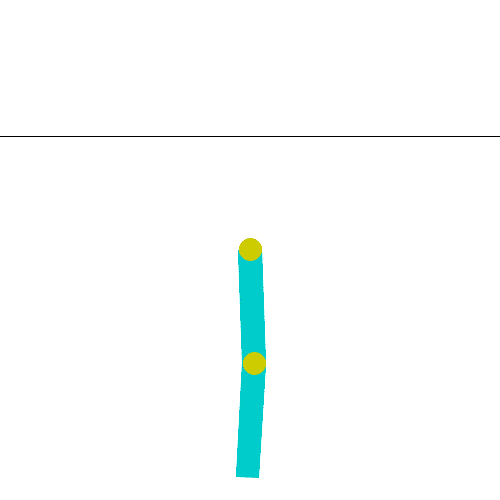
\includegraphics[width=0.4\textwidth]{acrobot} \hspace*{10mm} 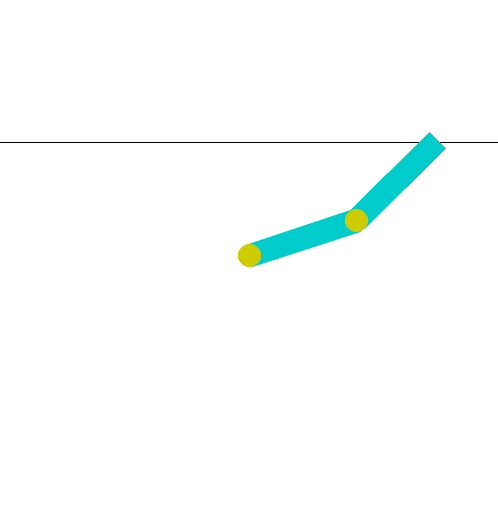
\includegraphics[width=0.4\textwidth]{acrobot_solved}
\caption[Illustration of the environment Acrobot]{
  \textbf{Illustration of the environment Acrobot.}
  The image on the left shows one possible state of the environment \texttt{Acrobot}. The image on the right shows one possibility of reaching the target height.
}
\label{fig:acrobot}
\end{figure}

\paragraph*{Action Space:} For \verb|Acrobot|, the action space is discrete and deterministic, representing the torque applied to the joint between the two links, including the loose end. Table~\ref{table:acrobot_act} shows a description of all possible actions.
\begin{table}[!ht]
  \centering
  \begin{tabular}{ |c|c|c| }
    \hline
    Action & Description & Unit \\
    \hline
    0 & apply -1 torque to the actuated joint & torque (N m) \\
    1 & apply 0 torque to the actuated joint & torque (N m) \\
    2 & apply 1 torque to the actuated joint & torque (N m) \\
    \hline
  \end{tabular}
  \caption[Action space of the environment Acrobot]{
    \textbf{Action space of the environment Acrobot.}
    Description of all possible actions for the \texttt{Acrobot} environment.
  }
  \label{table:acrobot_act}
\end{table}

\paragraph*{Observation Space:} \verb|Acrobot| returns six observations that inform us about the two rotational joint angles and their angular velocities. Table~\ref{table:acrobot_obs} contains a description for each observation. Here, \verb|theta1| is the angle of the first joint, where an angle of 0 indicates that the first link is pointing directly downwards; \verb|theta2| is relative to the angle of the first link. An angle of 0 corresponds to having the same angle between the two links.
\begin{table}[!ht]
  \centering
  \begin{tabular}{ |c|c|c| }
    \hline
    Observation & Min & Max \\
    \hline
    Cosine of \verb|theta1| & -1 & 1 \\
    Sine of \verb|theta1| & -1 & 1 \\
    Cosine of \verb|theta2| & -1 & 1 \\
    Sine of \verb|theta2| & -1 & 1 \\
    Angular velocity of \verb|theta1| & $\smallsim$ -12.567 (-4 * $\pi$) & $\smallsim$ 12.567 (4 * $\pi$) \\
    Angular velocity of \verb|theta2| & $\smallsim$ -28.274 (-9 * $\pi$) & $\smallsim$ 28.274 (9 * $\pi$) \\
    \hline
  \end{tabular}
  \caption[Observation space of the environment Acrobot]{
    \textbf{Observation space of the environment Acrobot.}
    Description of all observations for the \texttt{Acrobot} environment.
  }
  \label{table:acrobot_obs}
\end{table}

\paragraph*{Reward:} The goal of this task is to reach the target height with as few steps as possible. Thus, each step that does not attain the goal receives a negative reward of -1. Reaching the target height results in a reward of 0. An episode ends after 500 time steps. \verb|Acrobot| is considered an unsolved environment, meaning there is no reward threshold at which we would consider it solved.

\subsection{MountainCar and MountainCarContiuous}
The environments \verb|MountainCar| and \verb|MountainCarContiuous| are two different versions of the same problem. Both environments share the same observation space. The difference between the two is that \verb|MountainCar| has a discrete action space, and \verb|MountainCarContinuous| has a continuous action space. The goal of the task is to maneuver a car up a mountain to its target. However, the car's engine is not strong enough to drive up the slope in one push. To achieve the goal, we need to accelerate the car strategically. An agent should learn to swing from left to right to gain momentum and eventually reach the target. This task is rather difficult to learn since we counterintuitively need to move in the opposite direction of the target to swing up. The problem first appeared in Andrew Moore's PhD thesis \emph{Efficient memory-based learning for robot control} (\cite{moore1990efficient}). Fig~\ref{fig:mountain_car} shows one possible state in the left image and the target state of the two environments in the right image.
\begin{figure}[!ht]
  \centering
  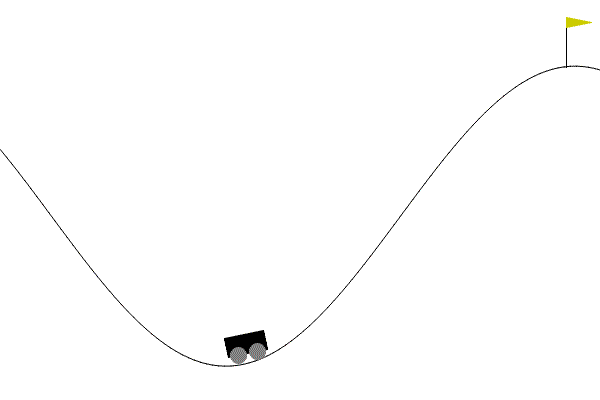
\includegraphics[width=0.4\textwidth]{mountain_car} \hspace*{10mm} 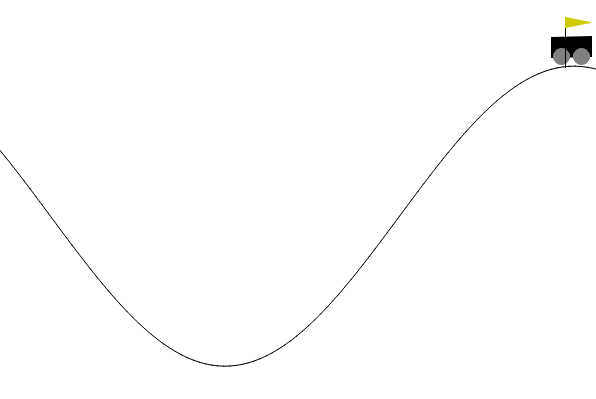
\includegraphics[width=0.4\textwidth]{mountain_car_solved}
\caption[Illustration of the environment MountainCar]{
  \textbf{Illustration of the environments MountainCar and MountainCarContinuous.}
  The image shows one possible state of the environments \texttt{MountainCar} and \texttt{MountainCarContiuous} on the left side. The image on the right shows the target state of the two environments.
}
\label{fig:mountain_car}
\end{figure}

\paragraph*{Action Space:} The action space for the environment \verb|MountainCar| consists of three discrete actions. We can accelerate the car to the right or the left, or we do not interact with it. The actions are further described in Table~\ref{table:mountaincar_act}.
\begin{table}[!ht]
  \centering
  \begin{tabular}{ |c|c|c|c| }
    \hline
    Action & Description \\
    \hline
    0 & Accelerate to the left \\
    1 & Don't accelerate  \\
    2 & Accelerate to the right \\
    \hline
  \end{tabular}
  \caption[Action space of the environment MountainCar]{
    \textbf{Action space of the environment MountainCar.}
    Description of all possible actions for the \texttt{MountainCar} environment.
  }
  \label{table:mountaincar_act}
\end{table}
On the other hand, the environment \verb|MountainCarContiuous| accepts one continuous action per step. The action represents the directional force on the car and is clipped in the range of [-1, 1] and multiplied by a power of 0.0015.

\paragraph*{Observation Space:} The environments \verb|MountainCar| and \verb|MountainCarContiuous| share the same observation space. They return two observations with information about the car's position and velocity. The observations are further described in Table~\ref{table:mountaincar_obs}.
\begin{table}[!ht]
  \centering
  \begin{tabular}{ |c|c|c|c| }
    \hline
    Observation & Min & Max \\
    \hline
    Position of the car along the x-axis & -1.2 & 0.6 \\
    Velocity of the car & -0.07 & 0.07 \\
    \hline
  \end{tabular}
  \caption[Observation space of the environment MountainCar]{
    \textbf{Observation space of the environment MountainCar.}
    Description of all observations for the \texttt{MountainCar} and \texttt{MountainCarContiuous} environments.
  }
  \label{table:mountaincar_obs}
\end{table}

\paragraph*{Reward:} To solve the task, the car has to reach the flag on the right hill as fast as possible. Each time step in which the agent cannot get to the target, it receives a negative reward of -1 for the environment \verb|MountainCar|. The task is considered solved when getting an average reward of at least -110.0 over 100 consecutive trials. For the environment \verb|MountainCarContiuous|, for each step in which the car does not reach the target, we receive a negative reward of
\[
  r = -0.1 * a^2,
\]
where $r$ is the reward and $a$ is the action. Like that, actions of large magnitude are penalized. When reaching the goal, we receive a positive reward of +100. The environment \texttt{MountainCarContiuous} is considered solved when getting an average reward of 90.0 over 100 consecutive trials.

\subsection{Pendulum}
For the environment \verb|Pendulum|, the system consists of a pendulum attached at one end to a fixed point and the other end being free. The goal is to apply torque on the fulcrum to swing it to an upright position. This task is known as the inverted pendulum swing-up problem and is based on the classic problem in control theory. Figure~\ref{fig:pendulum} shows one possible state of the environment in the left image and the target state in the right one.
 \begin{figure}[!ht]
  \centering
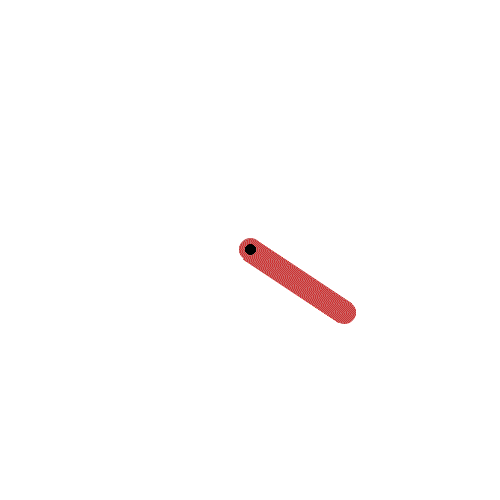
\includegraphics[width=0.4\textwidth]{pendulum} \hspace*{10mm}
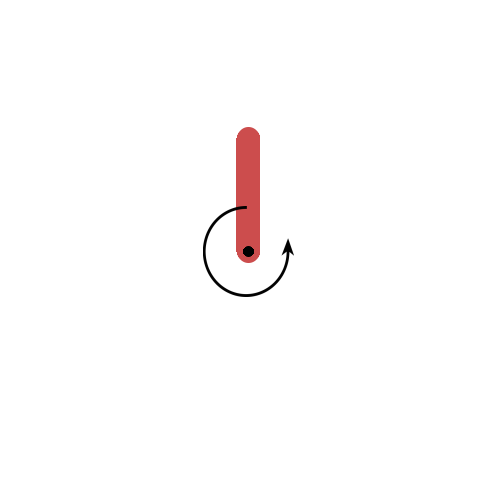
\includegraphics[width=0.4\textwidth]{pendulum_solved}
\caption[Illustration of the environment Pendulum]{
  \textbf{Illustration of the environment Pendulum.}
  The left image shows one possible state of the \texttt{Pendulum} environment. In the right image, the pendulum is in the upright position, which denotes the target state.
}
\label{fig:pendulum}
\end{figure}

\paragraph*{Action Space:} The environment accepts one action per step. The action represents the torque applied to the free end of the pendulum.
\begin{table}[!ht]
  \centering
  \begin{tabular}{ |c|c|c|c| }
    \hline
    Action & Description & Min & Max \\
    \hline
    0 & Torque & -2.0 & 2.0 \\
    \hline
  \end{tabular}
  \caption[Action space of the environment Pendulum]{
    \textbf{Action space of the environment Pendulum.}
    Description of all possible actions for the \texttt{Pendulum} environment.
  }
  \label{table:pendulum_act}
\end{table}

\paragraph*{Observation Space:} The environment returns three observations. The first two observations represent the x- and y-coordinate of the pendulum's free end in a cartesian coordinate system. The variable \verb|theta| defines the angle in radians. The third observation is the angular velocity of the free end of the pendulum.

\begin{table}[!ht]
  \centering
  \begin{tabular}{ |c|c|c| }
    \hline
    Observation & Min & Max \\
    \hline
    x = cos(\verb|theta|) & -1.0 & 1.0 \\
    y = sin(\verb|theta|) & -1.0 & 1.0 \\
    Angular Velocity & -8.0 & 8.0 \\
    \hline
  \end{tabular}
  \caption[Observation space of the environment Pendulum]{
    \textbf{Observation space of the environment Pendulum.}
    Description of all observations for the \texttt{Pendulum} environment.
  }
  \label{table:pendulum_obs}
\end{table}

\paragraph*{Reward:} The reward function is defined as $r = -(theta^2 + 0.1 * theta\_dt^2 + 0.001 * torque^2$). Regardless of the received reward, an episode ends after 200 time steps. \verb|Pendulum| is an unsolved environment meaning that it has no reward threshold at which we consider it solved.


\section{Analysis and Visualization}
\label{sec:benchmarks}
This thesis aims to deliver a proper analysis of different kinds of models in reinforcement learning. For this, we need appropriate methods and visualizations guaranteeing objectivity in evaluation.
 % When developing a novel algorithm, it is important to compare our results with existing models. For this evaluation, we need standard benchmark problems. These are a set of standard optimization problems. OpenAI Gym is a toolkit created for exactly this scenario. As mentioned in Section~\ref{sec:gym}, it contains a collection of benchmark problems with various levels of difficulty. However, not all benchmark problems are meaningful for the evaluation of an algorithm. If a problem is too trivial to solve, the results do not reflect the quality of the model adequately. We do not need to put a large amount of effort into the creation of a complex model for an easy-to-solve task.
\subsection{Reproducing Literature Results}
\cite{oller_analyzing_2020} deliver an excellent foundation for analysis in their paper \emph{Analyzing Reinforcement Learning Benchmarks with Random Weight Guessing}. The authors analyzed and visualized the complexity of standard reinforcement learning benchmarks based on score distribution.

They tested their approach on the five classic control benchmark problems from the OpenAI Gym interface discussed in Section~\ref{sec:environments}. The authors conducted a fixed series of experiments with each environment. They used three neural network architectures ($N_{architectures}=3$):
\begin{itemize}
  \item a network without any hidden layers (0 HL, 0 HU),
  \item a network with a single hidden layer of 4 units (1 HL, 4 HU),
  \item a network with two hidden layers of 4 units each (2 HL, 4 HU).
\end{itemize}
With these, they cover a variety of network models that are suited to solve the given tasks.

For the analysis, the authors did not train the network models. Instead, they chose the network weights from the standard normal distribution $\mathcal{N}(0,1)$ with RWG. This approach assures randomness and no directed learning. They initialized $10^4$ samples ($N_{samples}=10^4$) with different random weights. The authors chose such a large number of samples to draw meaningful statistical conclusions from their experiments. Each sample represents a neural network controller that maps observations to actions in the environment.
%Chapter~\ref{ch:experiments} aims to explore function approximators other than neural networks representing the controller.
The authors tested the controllers for each environment during 20 independent episodes ($N_{episodes}=20$). They saved the score in the score tensor $S$ for each episode. Algorithm~\ref{alg:environment-evaluation} illustrates the procedure with pseudocode.

\begin{algorithm}
\caption{Evaluation process taken from \cite{oller_analyzing_2020}}
\begin{algorithmic}[1]
\State Initialize environment
\State Create array $S$ of size $N_{architectures} \times N_{samples} \times N_{episodes}$
\For{$n = 1,2,...,N_{samples}$}
    \State Sample NN weights randomly from $\mathcal{N}(0,1)$
    \For{$e=1,2,...,N_{episodes}$}
      \State Reset the environment
      \State Run episode with NN
      \State Store episode reward in $S_{a,n,e}$
    \EndFor
\EndFor
\end{algorithmic}
\label{alg:environment-evaluation}
\end{algorithm}

The authors calculated the mean performance over all episodes from a sample and its variance for the analysis. These statistics can reveal how successful and stable the network models are in completing a task. A low mean value suggests that the controller struggles to complete the task. The variance gives us further insight into the score distribution. It illustrates how spread out the scores are from their respective mean score. A high value means that we have high variability. A controller is valuable if it can solve a specific task reliably and stable: a high value for the mean and a low value for the variance.

However, initializing a network with random weights should not create a stable controller. If this is the case, we can assume that the task to solve was too trivial and is not valuable for evaluation measurements. In the illustrations of the paper, the authors visualized their results with three plots: a log-scale histogram of the mean scores, a scatter plot of the sample scores, and a scatter plot of score variance over the mean score.

\paragraph*{Reproduction of the results:} I reproduced the results of the authors following the mentioned methodology. My findings for the environment \verb|CartPole| are displayed in Figure~\ref{fig:plots_reproduced}.
\begin{figure}[h]
\centering
\begin{subfigure}{\textwidth}
  \centering
  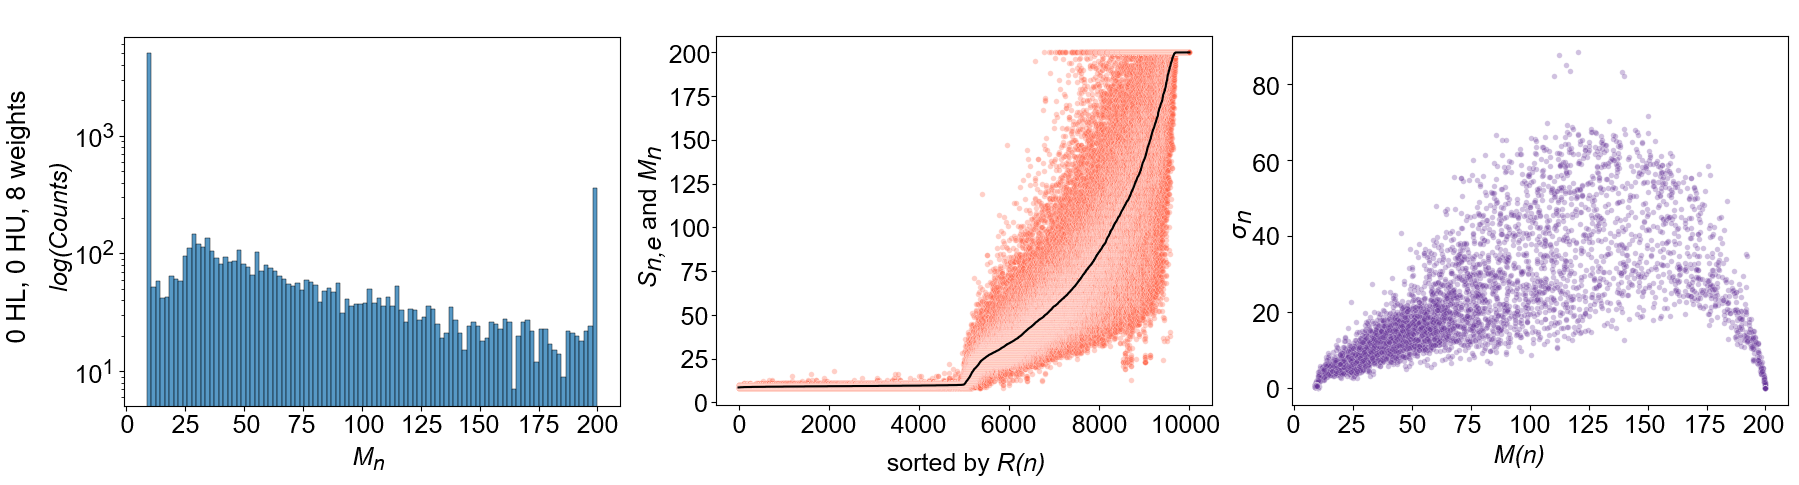
\includegraphics[width=\textwidth]{reproduced_plots/0_HL_0_HU}
    \caption{Results of the network architecture without hidden layers}
    \label{fig:plots_reproduced_first}
\end{subfigure}
\begin{subfigure}{\textwidth}
  \centering
  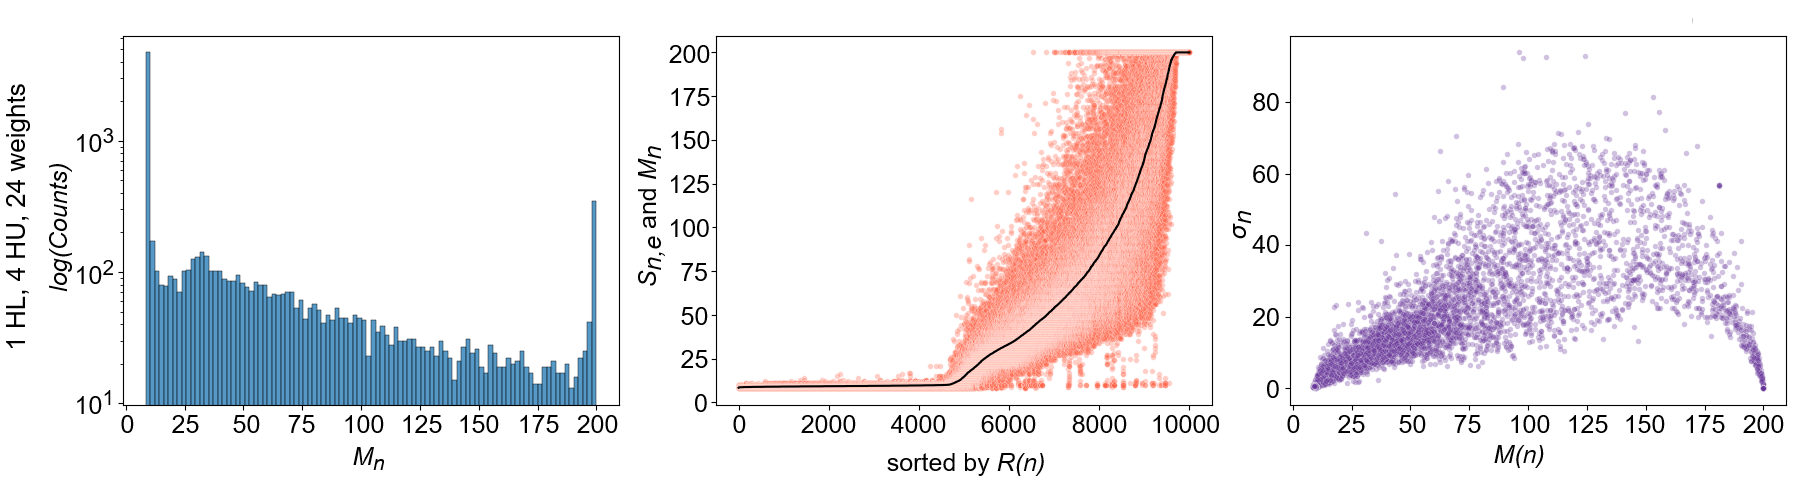
\includegraphics[width=\textwidth]{reproduced_plots/1_HL_4_HU}
    \caption{Results of the network architecture with one hidden layer}
    \label{fig:plots_reproduced_second}
\end{subfigure}
\begin{subfigure}{\textwidth}
  \centering
  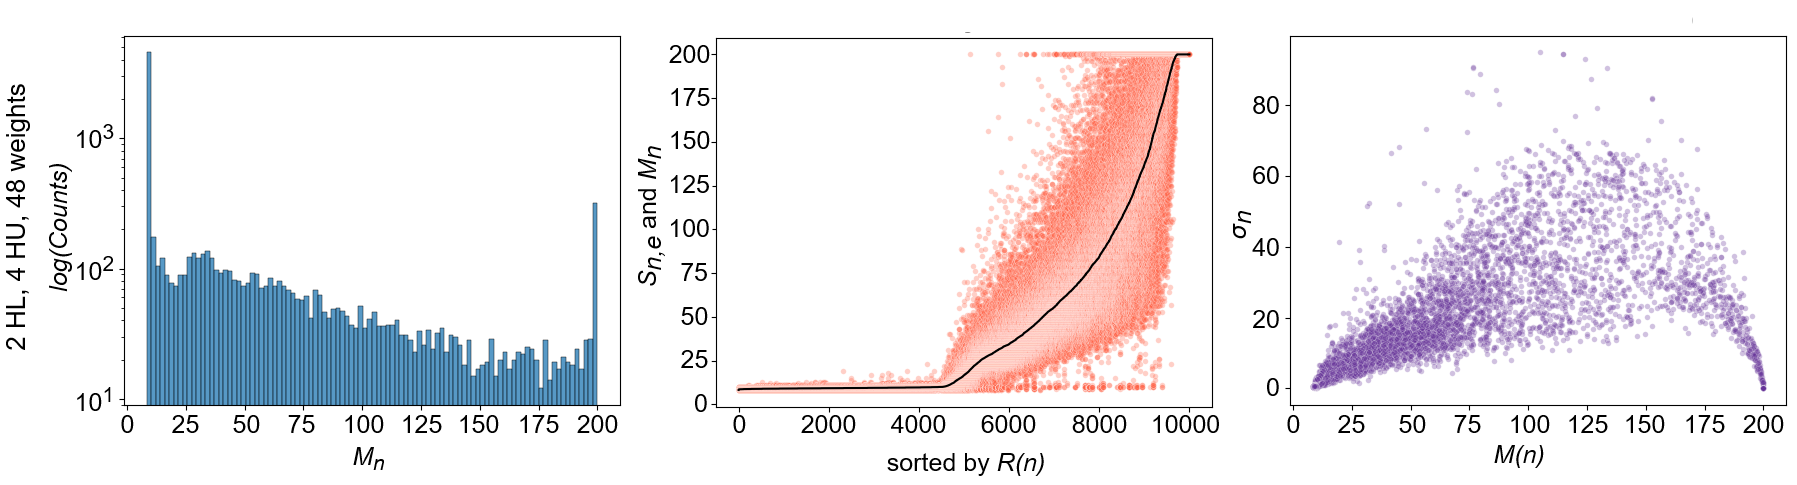
\includegraphics[width=\textwidth]{reproduced_plots/2_HL_4_HU}
    \caption{Results of the network architecture with two hidden layers}
    \label{fig:plots_reproduced_third}
\end{subfigure}
\caption[Results of the benchmark evaluation]{
  \textbf{Results of the benchmark evaluation.}
   The plots show a log-scale histogram of the mean scores (left images), a scatter plot of the sample scores over their rank (middle images), and a scatter plot of score variance over the mean score (right image). As expected with RWG, most networks could not solve the given task. However, a significant number of samples still achieve a mean score of 200. That suggests that the environment is trivial to solve.
}
\label{fig:plots_reproduced}
\end{figure}
The plots illustrate the results for each of the three network architectures. Each row shows the histogram of the mean score values in the first column, the scatter plot of all scores over their rank in the second column, and the scatter plot of the score variance over the mean score in the third column for the corresponding network architecture. There are few differences, but overall all network architectures deliver similar insights.

The histogram plots show that more than $10^3$ networks on the logarithmic scale receive a low score. A significant number of networks could still achieve a high mean value or the maximum value of 200. With a score of 200, the network solved the task in each episode. Therefore, the network could reliably solve the environment. Furthermore, in the scatter plots in the second column of Figure~\ref{fig:plots_reproduced}, we can see that the line plot of the mean scores is a continuous increasing line. A suited learning algorithm should generally be able to learn the task incrementally.

At the top of the scatter plots in the second column of Figure~\ref{fig:plots_reproduced}, we can see quite a few data points with a score of 200 that have a relatively low mean score. This behavior indicates that a network that generally performs poorly can still solve the task with the right initialization conditions. Lastly, in the scatter plots in the last column in Figure~\ref{fig:plots_reproduced}, we can see the distribution of the variance according to the mean value. On the left inside the scatter plots, we have low scores of variance corresponding with a low mean value. These networks were consistently unable to achieve a high score. We can expect most networks to be in this area without any training. However, the data points are spread out in the middle of the plot. For a high variance, the scores of a network differ highly from the mean value. Receiving a high score depends highly on the initialization conditions, meaning networks with this architecture are inconsistent and unstable. On the right inside the scatter plot, we can see that the data points with a high mean value are primarily of low variance. Thus, to achieve a high mean value, the network needs consistency.

\paragraph*{Impact of Bias:} Unexpectedly, but following the findings in \cite{oller_analyzing_2020}, the usage of the bias had a relatively significant impact on the performance of the network in my experiments. Without bias, the networks seem to achieve better scores overall. All plots in Figure~\ref{fig:plots_reproduced} illustrate the results without bias. For comparison, Figure~\ref{fig:comparison_bias} shows the results of a network with the same configurations as before, but this time including bias having a much lower score.
\begin{figure}[ht]
\centering
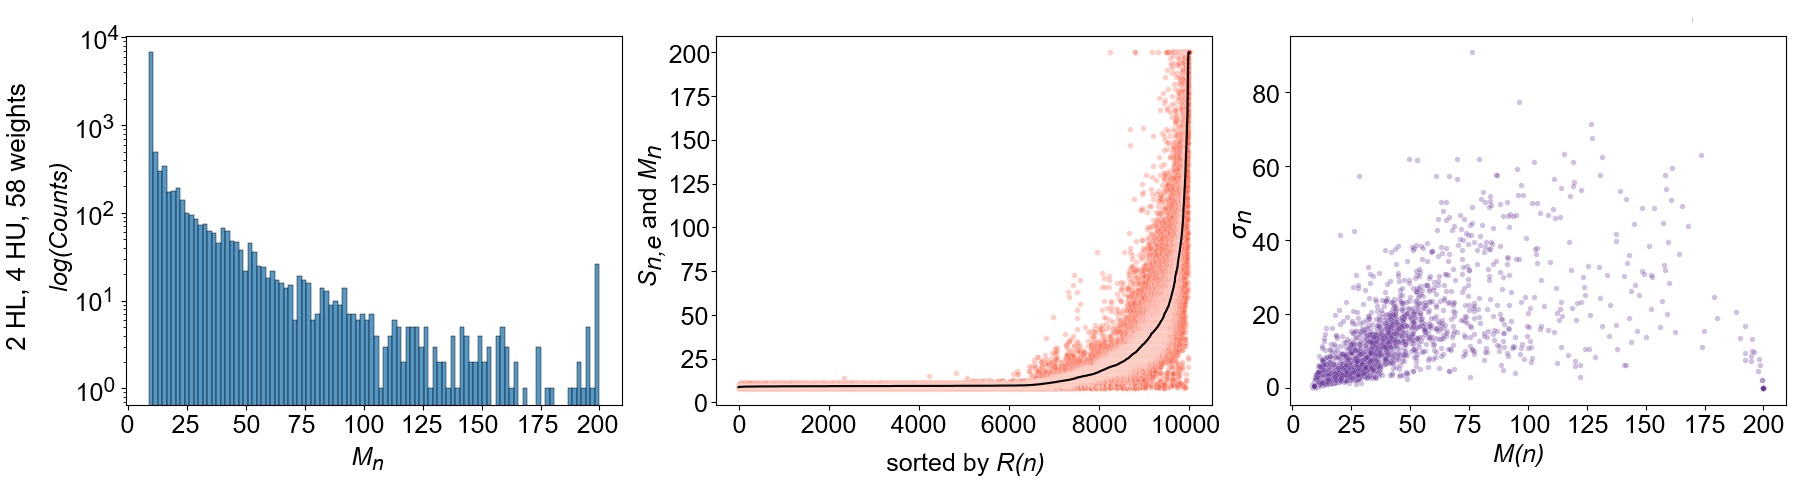
\includegraphics[width=1\textwidth]{with_bias_nn/2_HL_4_HU_bias}
\caption[Impact of bias]{
  \textbf{Impact of bias.}
  The figures show the performance of a network with two hidden layers with the same settings as before, but here we include bias. We can see that the network with bias connections performs much worse than those without bias connections.
}
\label{fig:comparison_bias}
\end{figure}
The number of networks that can consistently solve the task also decreases significantly. In the paper, the authors noted that the probability mass of top-performers generally increases when dropping the bias connections for all tested environments. Thus, this is not an isolated observation. However, they did not investigate this behavior further as it was not the focus of their paper.

One possible explanation could be that guessing additional weights might be fatal for achieving a good score. In other words: the more possibilities we have to guess a weight incorrectly, the higher the probability of failing. To test this hypothesis, we can alter the number of weights and compare the results. With an increased number of weights, we would expect the networks to perform worse than before. However, it could also be that the number of weights is not as impactful as the complexity of the model. Randomly guessing the parameters of a simple model has a higher chance of resulting in a good (simple) model than guessing the parameters of a more complex model.

The complexity of the network architecture gives an upper bound for the function that we can approximate. A network with high complexity maps into a larger search space with more complex functions. Since the size of the search space increases, there are also more possible samples that fail to solve the task. The paper showed that a simple model is sufficient to solve these environments. A complex model is oversized for our purpose here. Thus, randomly guessing a simple model can yield a model with good performance with enough attempts.

It is unlikely to randomly guess a complex model that performs well without any training involved. To test this hypothesis, we can increase the complexity of a network by varying the number of hidden layers or the number of neurons in a hidden layer. With increased complexity, we would expect the networks to perform worse than before.

Another interesting aspect would be to inspect the role of the bias in connection with the environments. A simple model is sufficient to solve a simple task. Nevertheless, what if the environment is more difficult to solve? In that case, the undersized complexity would limit us from finding an appropriate solution as the search space is not large enough for this scenario. Therefore, including bias should improve the results. That shows the importance of neural architecture search, a research field aiming to automate neural networks' architectural design process (\cite{DBLP:journals/corr/abs-2005-11074}).

Next to the analysis of the models, Chapter~\ref{ch:experiments} also contains the experiments following this thought process.

\subsection{Visualization}
For the visualization of the results, I am also following \cite{oller_analyzing_2020}. Figure~\ref{fig:plots_reproduced} already presented the type of plots used for the visualization in Chapter~\ref{ch:experiments}. However, I only use the scatter plots in the middle image because it transparently illustrates a high amount of information. Figure~\ref{fig:visualization} shows an example of such a plot.
\begin{figure}[!ht]
  \centering
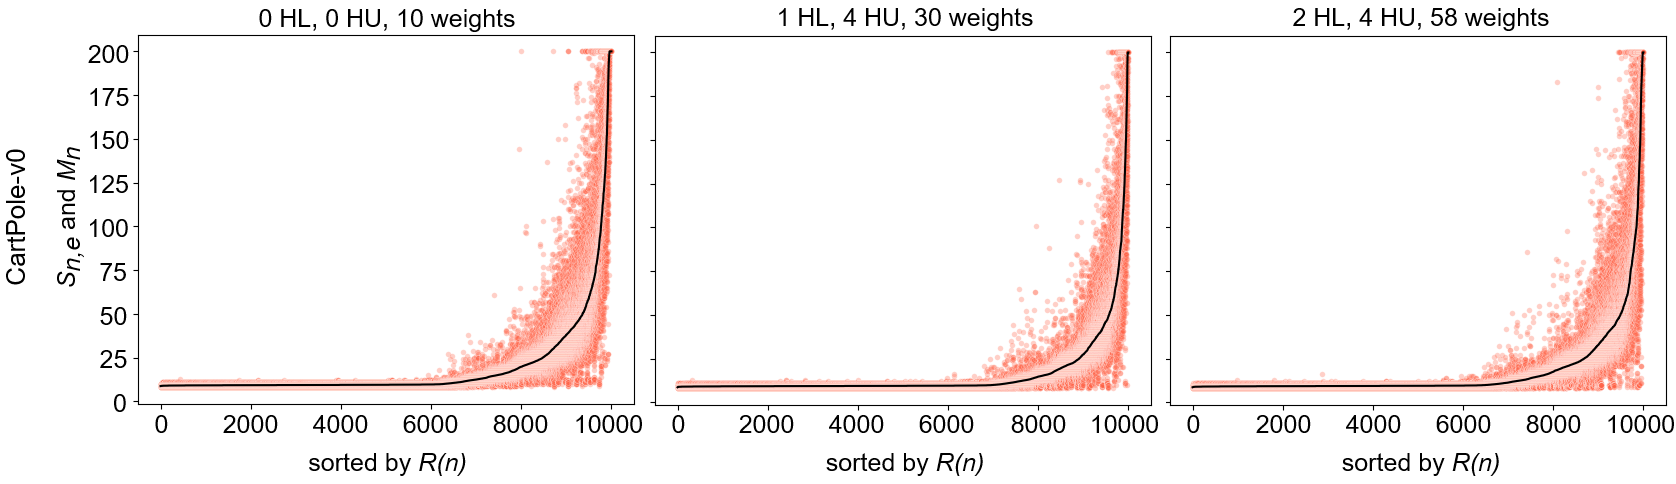
\includegraphics[width=\linewidth]{NN/NN_CartPole_new}
\caption[Visualization of results]{
  \textbf{Visualization of results.}
  The image shows an example of the visualization of the conducted experiments. The scatter plot represents the individual sample scores $S_{n,e}$ for episode $e$ over the rank $R(n)$ of the sample $n$. The overlaid line plot consists of each sample's mean scores $M_n$.
}
\label{fig:visualization}
\end{figure}
The different architectures of the model are aligned in the columns, and the row represents the environment. In this case, I am using three neural network architectures and the \verb|CartPole| environment. In each image, the samples are sorted according to their mean score for better analysis. The position of a sample $n$ within the sorted list is referred to as its rank $R(n)$. In the plot, the samples are aligned according to their rank on the x-axis. Each red dot represents the individual sample score $S_{n,e}$ for sample $n$ in episode $e$. The overlaid line plot represents the mean score $M_n$ of sample $n$ over all episodes. Thus, the line plot is a naturally increasing curve of the mean scores. The scatter plot indicates the variety of scores for one sample. The title of the plot informs us which model and how many weights were used. In addition, the corresponding OpenAI gym environment is declared.

%\todo[inline]{Maybe explain more.}

\section{Alternative Models}
\label{sec:models}
This section describes the models I used in the experiments. Since we are using black-box optimization techniques, we have no constraints on the model. Therefore, we can use any function approximator. Note that we are in the field of direct policy search, where we directly search in the search space of policies for a suited approximation.

\subsection{Polynomials}
Polynomials are equations in the form of a sum of powers in one or more variables multiplied by constant coefficients. Given a field $F$, a polynomial in variable $x$ with coefficients in $F$ is a formal expression denoted by
\begin{align*}
  &f(x) = \sum_{i=0}^{n} a_i x^i \in F[x], &a_0, ..., a_n \in F, \ \ i \in \mathbb{N},
\end{align*}
where $F[x]$ represents the set of all such polynomials (\cite{fischer2014}, p. 61). The above formula shows the one dimensional case. For the multi-dimensional case, $x$ and the coefficients are vectors instead of scalars. Thus, a polynomial $p(\mathbf{x})$ with $\mathbf{x} = [x_0, ..., x_m]^T$ being a vector and of degree $n$ can be represented by
\begin{align*}
  &p(\mathbf{x}) = \sum_{i=0}^{n} \mathbf{w_i}^T (x_k^i)_{k \in I} \in F^n[\mathbf{x}], &\mathbf{w_0}, ... \mathbf{w_n} \in F^n, \ \ I = \{0, ..., m\}.
\end{align*}
Polynomials are relatively simple mathematical expressions and their derivative and indefinite integral are easy to determine and are also polynomials. Due to their simple structure, polynomials can be valuable to analyze more complex functions using polynomial approximations. \textit{Taylor's theorem} tells us that we can locally approximate any $k$-times differentiable function by a polynomial of degree $k$. We call this approximation \textit{Taylor's polynomial}. Furthermore, the \textit{Weierstrass approximation theorem} says that we can uniformly approximate every continuous function defined on a closed interval by a polynomial. Other applications of polynomials are \textit{polynomial interpolation} and \textit{polynomial splines}. Polynomial interpolation describes the problem of constructing a polynomial that passes through all given data points. Polynomial splines are piecewise polynomial functions that can be used for spline interpolation. Spline interpolation is a form of interpolation where splines are used as interpolants.

\paragraph*{Construction of the model:} For the experiments with the polynomial model in Chapter~\ref{ch:experiments}, I constructed the model $P_1$. It consists of one polynomial mapping from the observaction space to the action space of the reinforcement learning environment for each possible action in a discrete action space. The dimension of the weight vectors is according to the dimension of the input vector. For example, for the environment \verb|CartPole| with the discrete action space $\{0, 1\}$ and observation $\mathbf{x} = [x_0, x_1, x_2, x_3]^T$, this means that $P_1$ consists of two polynomials:
\begin{align*}
  &p_0(\mathbf{x}) = \sum_{i=0}^{n} \mathbf{w_i}^T (x_k^i)_{k \in I} \in \mathbb{R}, &\mathbf{w_0}, ..., \mathbf{w_3}, \mathbf{x} \in \mathbb{R}^4, \ \ I = \{0, 1, 2, 3\} \\
  &p_1(\mathbf{x}) = \sum_{i=0}^{n} \mathbf{\hat{w}_i}^T (x_k^i)_{k \in I} \in \mathbb{R}, &\mathbf{\hat{w}_0}, ..., \mathbf{\hat{w}_3}, \mathbf{x} \in \mathbb{R}^4, \ \ I = \{0, 1, 2, 3\}
\end{align*}
In the formulas, $n$ denotes the degree of the polynomial. For the experiments, I used polynomials of degrees one, two, and three. However, the output of the polynomials is unbound, as illustrated in Figure~\ref{fig:bounds}. That makes it harder to interpret the results as probabilities.
\begin{figure}[ht]
\centering
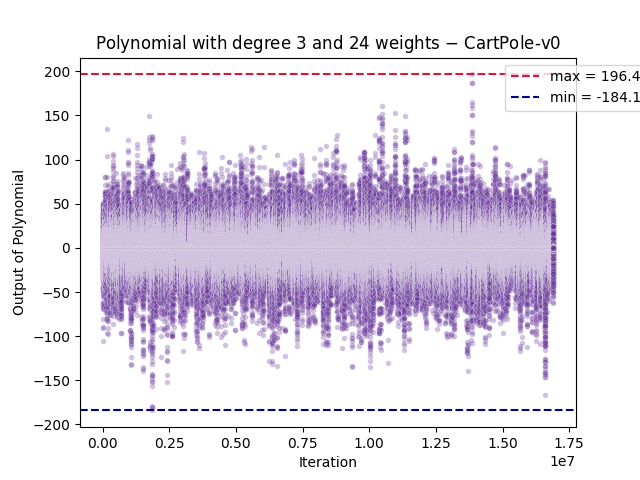
\includegraphics[width=0.6\textwidth]{PolynomialNN_degree_3_bounds}
\caption[Upper and lower bound]{
  \textbf{Upper and lower bound.}
  The figure shows each output of the polynomial functions described above. As we can see, the functions are not well bound, and there are quite a few outliers. That makes it hard to interpret the output sensibly.
}
\label{fig:bounds}
\end{figure}
So, I scaled the outputs with the logistic sigmoid function. We can interpret the output space of the sigmoid function as a probability, as discussed in Section~\ref{subsec:NN}. In this case, we search for the probability that a specific action is chosen given an observation $\mathbf{x}$. Thus, for our example with the \verb|CartPole| environment, we can interpret $sig(p_0)$ as the probability that action 0 is the correct one and $sig(p_1)$ as the probability that action 1 is the correct one. Putting this thought into a formula for $P_1$ and the \verb|CartPole| environment, we get:
\[
  P_1(\mathbf{x}) =
  \begin{cases}1~&{\text{ if }}~sig(p_1(\mathbf{x})) > sig(p_0(\mathbf{x}))~,\\0~&~\text{otherwise}~.\end{cases}
\]

% The second model $P_2$ is constructed similarly to $P_1$, but it only consists of one polynomial instead of one for each possible action. For the \verb|CartPole| environment, this means $P_2$ consists of:
% \[
%   p(\mathbf{x}) = \Sigma_{i=0}^{n} \mathbf{w_i}^T (x_k^i)_{k \in I} \in \mathbb{R}, \ \ \ \ \ \ \ \ \ \ \mathbf{w_i} \in \mathbb{R}^4, \ \ I = \{0, 1, 2, 3\}
% \]
% Analogous to $P_1$, I tested the polynomial $p(\mathbf{x})$ with degrees 1, 2, and 3. So, $n \in \{1, 2, 3\}$. In addition, I again used the logistic sigmoid function to scale the output of the polynomial. However, the output of $P_2$ is determined by a fixed threshold instead of comparing multiple polynomials. Putting this into a formula for the \verb|CartPole| environment, we get:
% \[
%   P_2(\mathbf{x}) =
%   \begin{cases}1~&{\text{ if }}~sig(p(\mathbf{x}))>0.5~,\\0~&~\text{otherwise}~.\end{cases}
% \]

% \subsection{Splines}
% General splines, adjustments \\ \\
% Splines can also be used as function approximators. However, with splines we do not aim to approximate the whole function but rather return a piecewise approximation.
%
% \todo[inline]{First was sind splines, dann herleitung in this case.}


\subsection{Binary Trees}
A binary tree is a common data type in computer science with a relatively simple design: a hierarchical tree structure consisting of a set of connected nodes. A node is a structure that can hold data and connections to other nodes, also called links or edges. Nodes in a binary tree have exactely two child nodes. A node's child nodes are those connected to it and situated beneath it in the tree. The node is then called the parent node in the perspective of its child nodes. Figure~\ref{fig:binary_tree_illustration} illustrates an example of a binary tree with seven nodes.
\begin{figure}[!ht]
\centering
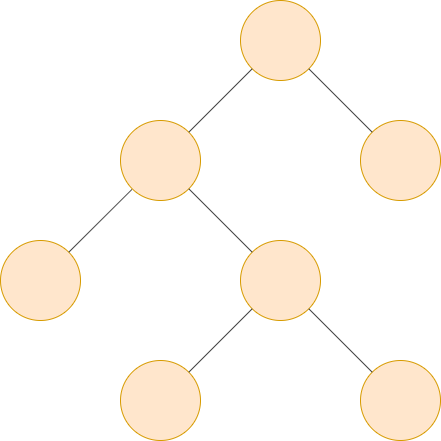
\includegraphics[width=0.4\textwidth]{binary_tree}
\caption[Example of a binary tree]{
  \textbf{Example of a binary tree.}
  The figure shows an example of a binary tree consisting of seven nodes.
}
\label{fig:binary_tree_illustration}
\end{figure}
The topmost node is called the root node. By design, there exists a path from the root node to every other node of the tree. The nodes which do not have child nodes are called leaf nodes.

We can use binary trees as decision trees for machine learning problems. Decision trees represent a predictive model to come to conclusions about a set of observations. For each node, we assess a feature, and a child node is selected accordingly. This process starts at the root node, and we repeat it until reaching a leaf node. The leaf node then holds the value of the target variable. In classification problems, the target variable takes on a value inside a discrete set of values. The leaves then represent the class labels. The target variable can also take on a constant value inside a specified range for regression problems.

The approach to decision trees is simple and intuitive when comparing them with other algorithms in machine learning. Decision trees split the input space into multiple partitions. When the dataset is splittable, it works well with fast predictions. Tree-based models like C4.5 which is an extension of the earlier ID3 algorithm and CART became quite popular (\cite{quinlan2014c4}; \cite{breiman2017classification}). C4.5 was even ranked one of the top ten algorithms in data mining (\cite{wu2008top}). Another advantage of decision trees is their interpretability since they implement rules humans can easily analyze. There were also approaches combining neural networks and decision trees. \cite{yang2018deep} introduced a neural network-based tree model DNDT which performed better for some datasets than neural networks while providing an interpretable decision process. Despite the success of decision trees in supervised learning problems, decision trees are not commonly used in reinforcement learning. Reinforcement learning introduces many challenges, including that the model has to constantly adapt as the interaction between the agent and the environment continues. \cite{silva2020optimization} approached this challenge by allowing for a gradient update over the entire tree.

\paragraph*{Construction of the model:} Since this study aims to experiment with models that will be optimized with black-box optimization techniques, we can use a simple binary tree model where each node holds three properties: \verb|values|, \verb|left|, \verb|right|. The variables \verb|left| and \verb|right| contain the two child nodes. If they are empty, the node is a leaf. The variable \verb|values| holds the model's output if the node is a leaf. Otherwise, it contains the weights used for the decision strategy. Figure~\ref{fig:binary_tree_model_illustration} illustrates the decision process of the binary tree model for the environment \verb|CartPole|.
\begin{figure}[!ht]
\centering
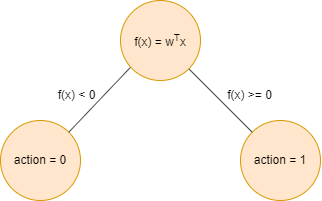
\includegraphics[width=0.5\textwidth]{binary_tree_model}
\caption[Illustration of binary tree model]{
  \textbf{Illustration of binary tree model.}
  The figure illustrates the binary tree model with the environment \texttt{CartPole}.
}
\label{fig:binary_tree_model_illustration}
\end{figure}
The illustrated model has one node for the decision finding and two leaf nodes containing the two possible discrete actions, 0 and 1. The dot product defines the decision-making process. For the environment \verb|CartPole| with observations $\mathbf{x} = [x_0, x_1, x_2, x_3]^T$, this results in the following formula:
\[
  f(\mathbf{x}) = \mathbf{w}^T\mathbf{x} = w_0 x_0 + w_1 x_1 + w_2 x_2 + w_3 x_3
\]
The variable $w$ represents the weights of the model. The actions of the leaves are fixed, whereas an optimization technique optimizes the weights of the nodes involved in the decision-making process.

The implementation is straightforward for environments like \verb|CartPole| where we only have two possible discrete actions. However, for an action space with more than two actions possible, the binary tree still has the same structure, but the decision is fixed between the minimum action and the maximum action. For example, for the environment \verb|Acrobot|, the minimum action is to apply -1 torque to the joint, and the maximum action is to apply 1 torque to the joint. In this case, we discard the action of applying 0 torque to the joint. Similarly, for environments with a continuous action space, we again take the minimum and the maximum of the value of the action. For the environment \verb|Pendulum|, this would be -2.0 and +2.0.

The only hyperparameter we have with this model is the number of nodes for the decision process. That makes hyperparameter tuning much more straightforward than it would be for other models like neural networks. Note that the leaves do not count as nodes for the model's architecture since each path in the tree has to result in a final decision between two actions. The leaf nodes are mandatory in that sense and thus cannot be altered in their number.

While simplistic, this model is easily extendable, for example, by having an equation decide the action in a leaf rather than a hardcoded action. Most importantly, architecture search using standard tree operators should be much more straightforward.

This thesis constitutes an initial feasibility study. So, further extensions are left to future work.

%\todo[inline]{Herleitung von splines erklären?}
